%%%%%%%%%%%%%%%%%%%%%%%%%%%%%%%%%%%%%%%%%%%%%%%%%%%%%%%%%%%%%%%%%%%%%%%%%%%%%%%
% CASE STUDY TEMPLATE - Programming and Problem Solving
% Author: Brendan Shea, PhD
% Course: Programming and Problem Solving
% Rochester Community and Technical College
%%%%%%%%%%%%%%%%%%%%%%%%%%%%%%%%%%%%%%%%%%%%%%%%%%%%%%%%%%%%%%%%%%%%%%%%%%%%%%%

\documentclass[11pt,letterpaper]{article}

%---------- PACKAGES ----------%
\usepackage[margin=1in, headheight=22pt]{geometry}
\usepackage[T1]{fontenc}
\usepackage{xcolor}
\usepackage{tcolorbox}
\usepackage{graphicx}
\usepackage{titlesec}
\usepackage{enumitem}
\usepackage{fancyhdr}
\usepackage{listings}
\usepackage{hyperref}
\usepackage{multicol}
\usepackage{booktabs}
\usepackage{tikz}
\usepackage{float}
\usepackage{amssymb}
\usepackage{amsmath}
\usepackage{pifont}

% TikZ libraries
\usetikzlibrary{shapes.geometric, arrows.meta, positioning, calc, backgrounds, fit, matrix, decorations.pathreplacing, chains}

% Load tcolorbox libraries
\tcbuselibrary{skins,breakable,listings,listingsutf8}

%---------- COLOR DEFINITIONS ----------%
\definecolor{csprimary}{HTML}{2C3E50}
\definecolor{cssecondary}{HTML}{E74C3C}
\definecolor{cstertiary}{HTML}{3498DB}
\definecolor{csaccent}{HTML}{27AE60}
\definecolor{cswarm}{HTML}{F39C12}
\definecolor{cslight}{HTML}{ECF0F1}
\definecolor{csdark}{HTML}{1A252F}

% Syntax highlighting colors
\definecolor{codegreen}{HTML}{27AE60}
\definecolor{codepurple}{HTML}{9B59B6}
\definecolor{codeorange}{HTML}{E67E22}
\definecolor{codeblue}{HTML}{3498DB}
\definecolor{codegray}{HTML}{95A5A6}
\definecolor{codestring}{HTML}{E74C3C}
\definecolor{codebg}{HTML}{1E2A38}

%---------- CASE STUDY METADATA ----------%
\newcommand{\cstitle}{From Text Files to AI Agents}
\newcommand{\cssubtitle}{The Rise (and Transformation) of the Developer Environment}
\newcommand{\csauthor}{Brendan Shea, PhD}
\newcommand{\cscourse}{Programming and Problem Solving}
\newcommand{\csinstitution}{Rochester Community and Technical College}
\newcommand{\csdate}{\today}

%---------- LISTINGS CONFIGURATION ----------%
\lstdefinestyle{basestyle}{
    backgroundcolor=\color{codebg},
    basicstyle=\ttfamily\small\color{white},
    breakatwhitespace=false,
    breaklines=true,
    captionpos=b,
    keepspaces=true,
    showspaces=false,
    showstringspaces=false,
    showtabs=false,
    tabsize=4,
    frame=none,
    xleftmargin=4mm,
    xrightmargin=4mm,
    aboveskip=0pt,
    belowskip=0pt,
}

\lstdefinestyle{javastyle}{
    style=basestyle,
    language=Java,
    keywordstyle=\color{codeblue}\bfseries,
    commentstyle=\color{codegray}\itshape,
    stringstyle=\color{codestring},
    morekeywords={String, Scanner, System, var, boolean, Math, List, Map, HashMap, ArrayList},
}

\lstdefinestyle{bashstyle}{
    style=basestyle,
    language=bash,
    keywordstyle=\color{codeblue}\bfseries,
    commentstyle=\color{codegray}\itshape,
    stringstyle=\color{codestring},
}

%---------- CUSTOM ENVIRONMENTS ----------%
\newcommand{\keyterm}[1]{\textbf{\textcolor{cssecondary}{#1}}}

\newtcolorbox{conceptbox}[1][]{
    enhanced,
    colback=cslight,
    colframe=csprimary,
    fonttitle=\bfseries\color{white},
    title=#1,
    attach boxed title to top left={yshift=-2mm, xshift=5mm},
    boxed title style={colback=csprimary},
    breakable
}

\newtcolorbox{historybox}[1][]{
    enhanced,
    colback=codepurple!8,
    colframe=codepurple,
    fonttitle=\bfseries\color{white},
    title=#1,
    attach boxed title to top left={yshift=-2mm, xshift=5mm},
    boxed title style={colback=codepurple},
    breakable
}

\newtcolorbox{tipbox}[1][]{
    enhanced,
    colback=csaccent!8,
    colframe=csaccent,
    fonttitle=\bfseries\color{white},
    title=#1,
    attach boxed title to top left={yshift=-2mm, xshift=5mm},
    boxed title style={colback=csaccent},
    breakable
}

\newtcolorbox{debatebox}[1][]{
    enhanced,
    colback=cswarm!8,
    colframe=cswarm,
    fonttitle=\bfseries\color{white},
    title=#1,
    attach boxed title to top left={yshift=-2mm, xshift=5mm},
    boxed title style={colback=cswarm},
    breakable
}

\newtcolorbox{quotebox}[1][]{
    enhanced,
    colback=cstertiary!8,
    colframe=cstertiary,
    fonttitle=\bfseries\color{white},
    title=#1,
    attach boxed title to top left={yshift=-2mm, xshift=5mm},
    boxed title style={colback=cstertiary},
    breakable
}

\newtcblisting{javacode}[1][]{
    enhanced,
    colback=codebg,
    colframe=csaccent,
    colupper=white,
    fonttitle=\bfseries\color{white},
    title=#1,
    attach boxed title to top left={yshift=-2mm, xshift=5mm},
    boxed title style={colback=csaccent},
    left=0mm, right=0mm, top=2mm, bottom=2mm,
    boxrule=1pt,
    breakable,
    pad at break=2mm,
    listing only,
    listing options={style=javastyle}
}

\newtcblisting{bashcode}[1][]{
    enhanced,
    colback=codebg,
    colframe=codepurple,
    colupper=white,
    fonttitle=\bfseries\color{white},
    title=#1,
    attach boxed title to top left={yshift=-2mm, xshift=5mm},
    boxed title style={colback=codepurple},
    left=0mm, right=0mm, top=2mm, bottom=2mm,
    boxrule=1pt,
    breakable,
    pad at break=2mm,
    listing only,
    listing options={style=bashstyle}
}

\newtcolorbox{questionbox}{
    enhanced,
    colback=cswarm!10,
    colframe=cswarm,
    fonttitle=\bfseries\color{white},
    title=Discussion Questions,
    attach boxed title to top center={yshift=-2mm},
    boxed title style={colback=cswarm},
    breakable
}

\newtcolorbox{glossarybox}{
    enhanced,
    colback=cslight,
    colframe=csprimary,
    fonttitle=\bfseries\color{white},
    title=Glossary of Key Terms,
    attach boxed title to top center={yshift=-2mm},
    boxed title style={colback=csprimary},
    breakable
}

%---------- HEADER/FOOTER ----------%
\pagestyle{fancy}
\fancyhf{}
\fancyhead[L]{\small\textcolor{csprimary}{\cscourse}}
\fancyhead[R]{\small\textcolor{csprimary}{Case Study}}
\fancyfoot[C]{\thepage}
\renewcommand{\headrulewidth}{0.4pt}
\renewcommand{\headrule}{\hbox to\headwidth{\color{csprimary}\leaders\hrule height \headrulewidth\hfill}}

%---------- SECTION FORMATTING ----------%
\titleformat{\section}
    {\Large\bfseries\color{csprimary}}
    {\thesection}{1em}{}[\color{cssecondary}\titlerule]

\titleformat{\subsection}
    {\large\bfseries\color{cstertiary}}
    {\thesubsection}{1em}{}

%---------- HYPERLINK SETTINGS ----------%
\hypersetup{
    colorlinks=true,
    linkcolor=cstertiary,
    urlcolor=cstertiary
}

%%%%%%%%%%%%%%%%%%%%%%%%%%%%%%%%%%%%%%%%%%%%%%%%%%%%%%%%%%%%%%%%%%%%%%%%%%%%%%%
\begin{document}

%---------- TITLE BLOCK ----------%
\begin{tcolorbox}[
    enhanced,
    colback=csprimary,
    colframe=csprimary,
    arc=0mm,
    left=10mm, right=10mm, top=8mm, bottom=8mm
]
\begin{center}
    {\huge\bfseries\color{white}\cstitle}\\[3mm]
    {\Large\color{cslight}\cssubtitle}\\[5mm]
    \textcolor{cssecondary}{\rule{0.5\textwidth}{1pt}}\\[5mm]
    {\large\color{white}\csauthor}\\[2mm]
    {\normalsize\color{cslight}\cscourse\ $\bullet$ \csinstitution}
\end{center}
\end{tcolorbox}

\vspace{5mm}

%---------- INTRODUCTION ----------%
\section*{Introduction}

When you open VS Code today, you're greeted with syntax highlighting, instant error underlining, auto-complete suggestions, an integrated terminal, and a sidebar full of file management tools---all before you've typed a single character. It's easy to take for granted. But this sophisticated environment represents decades of innovation. And right now, it's undergoing its most radical transformation yet.

For most of computing history, writing code meant working directly with plain text files and running commands in a terminal. Then came the \keyterm{Integrated Development Environment} (IDE)---software designed to put everything a programmer needs in one place. IDEs became so dominant that most programmers today have never worked without one.

But the rise of \keyterm{AI coding assistants} and \keyterm{agent interfaces}---tools where you describe what you want and an AI writes, edits, and runs the code---is raising a new question: what is the IDE \textit{for}, and what will replace it? This case study traces that arc from the command line to the agent, and explains what it means for you as a beginning programmer.

\begin{conceptbox}[Three Eras of Developer Tooling]
\textbf{Era 1 --- The Text File Era (1960s--1980s):} Programmers edit plain text, compile manually, and debug with print statements. The terminal is the entire environment.

\textbf{Era 2 --- The IDE Era (1990s--2010s):} All-in-one applications bundle editing, compilation, debugging, and project management. The programmer is in control; the IDE assists.

\textbf{Era 3 --- The Agent Era (2020s--present):} AI systems can read, write, and run code autonomously. The programmer increasingly acts as a director, reviewer, and guide---rather than the sole author.

None of these eras has ended. Text editors still exist. IDEs are thriving. And agents are just getting started.
\end{conceptbox}

%---------- ERA 1: THE TEXT FILE ----------%
\section{Era 1: Plain Text and the Command Line}

\subsection{What ``Writing Code'' Once Meant}

In the early decades of computing---the 1960s, 70s, and 80s---writing a program meant creating a plain text file and then \textit{manually} running a series of commands to turn that text into something the computer could execute. There was no graphical interface, no color-coded text, no built-in spell-check for your syntax. Just you, a terminal (or even a physical punch-card machine), and a blinking cursor.

\begin{historybox}[The Punch Card Era]
Before video terminals became common, many programmers wrote code on physical punch cards---stiff paper cards where holes represented characters. A program might be a stack of hundreds of cards, each representing one line of code. If you dropped the stack and shuffled the order, you had to sort them by hand.

By the late 1970s, video terminals replaced punch cards, and programmers typed directly into text editors like \texttt{ed} (1969) and later \texttt{vi} (1976). These tools are still available on almost every Unix and Linux system today---and still used by experienced developers.
\end{historybox}

The workflow of a 1980s programmer looked something like this:

\begin{bashcode}[A Typical 1980s Workflow]
# 1. Write source code in a text editor
vi HelloWorld.java

# 2. Save the file and exit the editor

# 3. Compile manually
javac HelloWorld.java

# 4. If there are errors, read them in the terminal,
#    go back to the editor, find the line, fix it, repeat

# 5. Run the program
java HelloWorld

# 6. If the output is wrong, add print statements to debug
\end{bashcode}

This process---write, compile, read errors, fix, repeat---is called the \keyterm{edit-compile-run cycle}. It's still the fundamental loop of programming today. The tools around it have changed enormously; the loop itself has not.

\subsection{The Text Editors That Survived}

Two text editors from this era are worth knowing about because they're still actively used and you'll encounter them on servers, in tutorials, and in job interviews.

\begin{center}
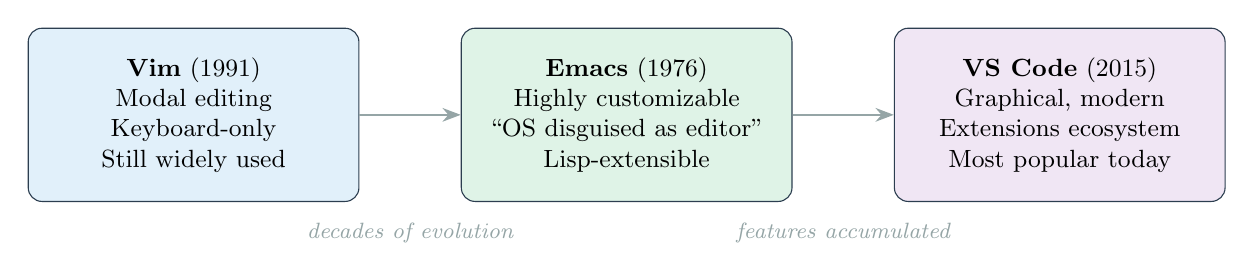
\begin{tikzpicture}[
    tool/.style={rectangle, rounded corners=5pt, draw=csprimary, fill=#1, minimum width=42mm, minimum height=22mm, align=center, font=\small},
]
\node[tool=cstertiary!15] (vim) at (0,0) {\textbf{Vim} (1991)\\\small Modal editing\\\small Keyboard-only\\\small Still widely used};
\node[tool=csaccent!15] (emacs) at (5.5,0) {\textbf{Emacs} (1976)\\\small Highly customizable\\\small ``OS disguised as editor''\\\small Lisp-extensible};
\node[tool=codepurple!15] (vscode) at (11,0) {\textbf{VS Code} (2015)\\\small Graphical, modern\\\small Extensions ecosystem\\\small Most popular today};

\draw[-{Stealth}, thick, color=codegray] (vim.east) -- (emacs.west);
\draw[-{Stealth}, thick, color=codegray] (emacs.east) -- (vscode.west);

\node[font=\footnotesize\itshape, color=codegray] at (2.75,-1.5) {decades of evolution};
\node[font=\footnotesize\itshape, color=codegray] at (8.25,-1.5) {features accumulated};
\end{tikzpicture}
\end{center}

\textbf{Vim} uses a \keyterm{modal editing} model: the editor has different modes for inserting text, navigating, and running commands. It looks confusing at first (\textit{how do I quit this thing?}) but its keyboard shortcuts let experienced users edit text very fast without ever touching a mouse. On any Linux server you'll ever access---a cloud virtual machine, a production system, a Raspberry Pi---Vim will be there.

\begin{tipbox}[Practical Tip: Learning Basic Vim]
You don't need to master Vim, but knowing the basics will save you in situations where it's the only option (like editing a file on a remote server). Key commands:
\begin{itemize}[itemsep=2pt]
    \item \texttt{i} --- enter Insert mode (start typing)
    \item \texttt{Esc} --- return to Normal mode
    \item \texttt{:w} --- save the file
    \item \texttt{:q} --- quit (use \texttt{:wq} to save and quit, \texttt{:q!} to quit without saving)
    \item \texttt{/word} --- search for ``word''
\end{itemize}
Run \texttt{vimtutor} in any terminal for a built-in 30-minute interactive lesson.
\end{tipbox}

\subsection{What Was Missing}

Working with plain text editors and manual compilation worked, but it was slow and error-prone. Every typo was discovered only after compilation. Navigating large projects meant remembering file names. Debugging required inserting \texttt{System.out.println()} calls everywhere and recompiling. Refactoring---renaming a variable used in twenty files---was a manual, error-prone process.

Programmers knew things could be better. The tools that would emerge to solve these problems would reshape the profession.

%---------- ERA 2: THE RISE OF THE IDE ----------%
\section{Era 2: The Rise of the Integrated Development Environment}

\subsection{What an IDE Actually Is}

An \keyterm{Integrated Development Environment} combines, in a single application, the tools a programmer needs to write, run, and debug software. The word ``integrated'' is key: instead of separately invoking a text editor, a compiler, a debugger, and a file manager from the command line, all of these live together in one interface.

\begin{historybox}[Early IDEs: Turbo Pascal and Visual Basic]
The first widely successful IDEs appeared in the late 1980s and early 1990s. \textbf{Turbo Pascal} (Borland, 1983) was a revelation: you could write code, compile it, and run it from the same screen, and compilation was so fast it happened almost instantly. Many programmers encountered it as their first taste of an integrated environment.

\textbf{Visual Basic} (Microsoft, 1991) went further, adding a visual form designer: you could drag and drop buttons and text fields onto a window, and Visual Basic would generate the code for you. For beginners, seeing an application appear on screen with minimal code was genuinely exciting---and it introduced millions of people to programming.
\end{historybox}

By the 2000s, two IDEs dominated:

\begin{itemize}[itemsep=4pt]
    \item \textbf{Eclipse} (IBM, open-sourced 2001): A free, extensible IDE for Java that became the standard in enterprise development and universities. Heavy but powerful.
    \item \textbf{IntelliJ IDEA} (JetBrains, 2001): A commercial IDE with exceptional Java support. IntelliJ's ``smart'' features---deep code analysis, powerful refactoring---set a new standard for what an IDE could do.
\end{itemize}

Today, \textbf{Visual Studio Code} (Microsoft, 2015) is the most widely used editor in the world. It occupies a middle ground: lighter than Eclipse or IntelliJ, richer than plain text editors, and extensible through thousands of community-built plugins.

\subsection{The Features That Changed Everything}

What do IDEs provide that plain text editors don't? Several features that, once you've used them, feel indispensable:

\begin{center}
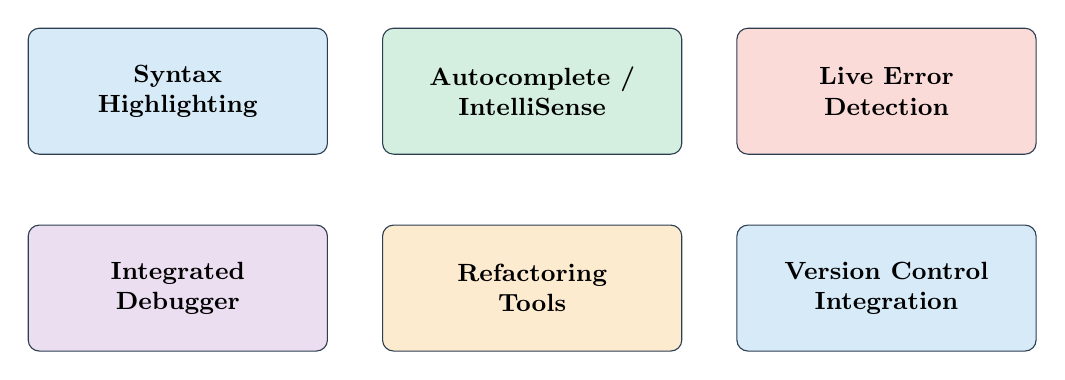
\begin{tikzpicture}[
    feature/.style={rectangle, rounded corners=4pt, draw=csprimary, fill=#1, minimum width=38mm, minimum height=16mm, align=center, font=\small\bfseries},
    label/.style={font=\footnotesize, color=codegray, align=center}
]

\node[feature=cstertiary!20] (sh) at (0,2.5) {Syntax\\Highlighting};
\node[feature=csaccent!20] (ac) at (4.5,2.5) {Autocomplete /\\IntelliSense};
\node[feature=cssecondary!20] (err) at (9,2.5) {Live Error\\Detection};
\node[feature=codepurple!20] (dbg) at (0,0) {Integrated\\Debugger};
\node[feature=cswarm!20] (ref) at (4.5,0) {Refactoring\\Tools};
\node[feature=cstertiary!20] (vcs) at (9,0) {Version Control\\Integration};

\end{tikzpicture}
\end{center}

\textbf{Syntax highlighting} colors keywords, strings, and variables differently, making code far easier to read at a glance. This sounds minor but has a profound effect on comprehension---your eye immediately catches a mismatched quote or an unrecognized keyword.

\textbf{Autocomplete} (called \keyterm{IntelliSense} in VS Code) suggests method names, variable names, and parameters as you type. For a beginning programmer, this is enormously helpful: you don't need to memorize every method name, just the first few characters. For an expert, it eliminates tedious typing.

\begin{javacode}[What IntelliSense Does For You]
// You type:
String message = "Hello, world!";
message.

// IntelliSense immediately shows a dropdown:
//   charAt(int index)
//   contains(CharSequence s)
//   indexOf(String str)
//   length()
//   substring(int beginIndex)
//   toUpperCase()
//   ... and 40 more methods

// You don't need to remember the exact name.
// You pick from the list.
\end{javacode}

\textbf{Live error detection} underlines mistakes as you type---before you even try to compile. A red squiggle under a missing semicolon or a misspelled variable name means you fix problems immediately rather than discovering them minutes later during compilation.

\textbf{The integrated debugger} is perhaps the most powerful feature. Instead of adding print statements to understand what your code is doing, you can set a \keyterm{breakpoint}---a marker telling the debugger to pause execution at that line. When the program pauses, you can inspect every variable's value, step through code line by line, and understand exactly what is happening.

\begin{tipbox}[Practical Tip: Use the Debugger Instead of Print Statements]
New programmers often debug by adding \texttt{System.out.println()} everywhere. This works, but it's slow and clutters your code. Learn to use the debugger in VS Code instead:
\begin{enumerate}[itemsep=2pt]
    \item Click in the margin next to a line number to set a breakpoint (a red dot appears)
    \item Run your program in ``Debug'' mode (F5 in VS Code)
    \item When the program hits your breakpoint, it pauses
    \item Check the ``Variables'' panel to see every variable's current value
    \item Press F10 to step to the next line, F11 to step \textit{into} a method call
\end{enumerate}
This skill separates programmers who struggle with bugs from those who solve them quickly.
\end{tipbox}

\subsection{Version Control Integration}

Modern IDEs also integrate with \keyterm{version control} systems, particularly \keyterm{Git}. Git tracks every change you make to your code over time, allowing you to:

\begin{itemize}[itemsep=3pt]
    \item Revert to any previous version if you break something
    \item See exactly what changed between two versions
    \item Collaborate with others without overwriting each other's work
    \item Maintain multiple experimental versions (``branches'') simultaneously
\end{itemize}

VS Code shows which lines have been added, changed, or deleted since your last Git commit, right in the editor margin. You can stage changes, write commit messages, and push to GitHub without leaving the editor.

\begin{tipbox}[Practical Tip: Commit Early and Often]
Beginning programmers often make many changes before committing to Git---then have trouble remembering what they changed and why. The habit to build: commit small, logical units of work with clear messages.

\begin{itemize}[itemsep=2pt]
    \item Bad message: ``stuff''
    \item Bad message: ``fixed it''
    \item Good message: ``Fix off-by-one error in loop that counted array elements''
    \item Good message: ``Add input validation to prevent negative grades''
\end{itemize}
Future you---trying to understand why the code is the way it is---will be grateful.
\end{tipbox}

\subsection{Why IDEs Won}

The IDE model succeeded because it dramatically reduced the cognitive overhead of programming. You could focus on solving the problem at hand rather than managing the toolchain. Errors surfaced immediately. Navigation in large codebases became manageable. And the visual debugger made understanding runtime behavior vastly easier than staring at print output.

By the 2010s, the question wasn't ``should I use an IDE?'' but ``which IDE?'' The era of the plain text editor, for most programmers doing most work, was over.

%---------- ERA 3: AI ENTERS THE EDITOR ----------%
\section{Era 3: AI Enters the Editor}

\subsection{The First Wave: Autocomplete Gets Smarter}

The IDEs of the 2010s were good, but their autocomplete was still fundamentally mechanical: it looked up names in the current codebase and standard library. It couldn't suggest that you needed a loop here, or that you probably wanted to handle the null case, or that there was a smarter way to solve this problem.

That changed in 2021 when GitHub released \keyterm{GitHub Copilot}, powered by OpenAI's Codex model. Copilot had been trained on billions of lines of publicly available code, and it could do something unprecedented: given a comment describing what you wanted, it would generate plausible working code.

\begin{javacode}[Copilot-Style AI Completion (2021)]
// Calculate the average of a list of integers,
// ignoring negative values
public double averagePositive(List<Integer> numbers) {
    // <- cursor here; AI suggests the entire method body:

    return numbers.stream()
        .filter(n -> n > 0)
        .mapToInt(Integer::intValue)
        .average()
        .orElse(0.0);
}
\end{javacode}

This was qualitatively different from traditional autocomplete. The AI wasn't looking up a method name---it was generating novel code based on understanding what the comment described.

\begin{historybox}[From Codex to Copilot to Cursor]
\textbf{2021}: GitHub Copilot launches as an IDE extension, offering AI-powered code completion inside VS Code and other editors.

\textbf{2022--2023}: The release of ChatGPT makes LLMs a mainstream phenomenon. Programmers start asking ChatGPT to explain errors, generate boilerplate, and suggest implementations---copy-pasting between the browser and their editor.

\textbf{2023}: \textbf{Cursor} launches---an editor \textit{built around} AI. Rather than bolting AI onto VS Code, Cursor integrates AI deeply: you can select code and ask the AI to rewrite it, explain it, or fix it. The AI can see your entire codebase, not just the current file.

\textbf{2024}: Major IDEs (VS Code, JetBrains) add their own native AI features. The question shifts from ``should I use AI?'' to ``which AI integration works best?''

\textbf{2025}: AI agents---systems that can autonomously run code, read files, search the web, and make changes across an entire codebase---move from research experiments to practical tools.
\end{historybox}

\subsection{The Agent Interface: A Different Paradigm}

AI code assistants inside editors still follow the IDE model: you, the programmer, are at the center, making every decision. The AI is a very capable autocomplete. But \keyterm{AI coding agents} represent something more fundamental.

An agent doesn't just suggest the next line---it can:
\begin{itemize}[itemsep=3pt]
    \item Read your entire codebase to understand context
    \item Write new files or edit existing ones
    \item Run your tests and interpret the results
    \item Search the web for documentation or examples
    \item Execute code, observe output, and fix errors it finds
    \item Perform multi-step tasks spanning many files and many minutes
\end{itemize}

\begin{center}
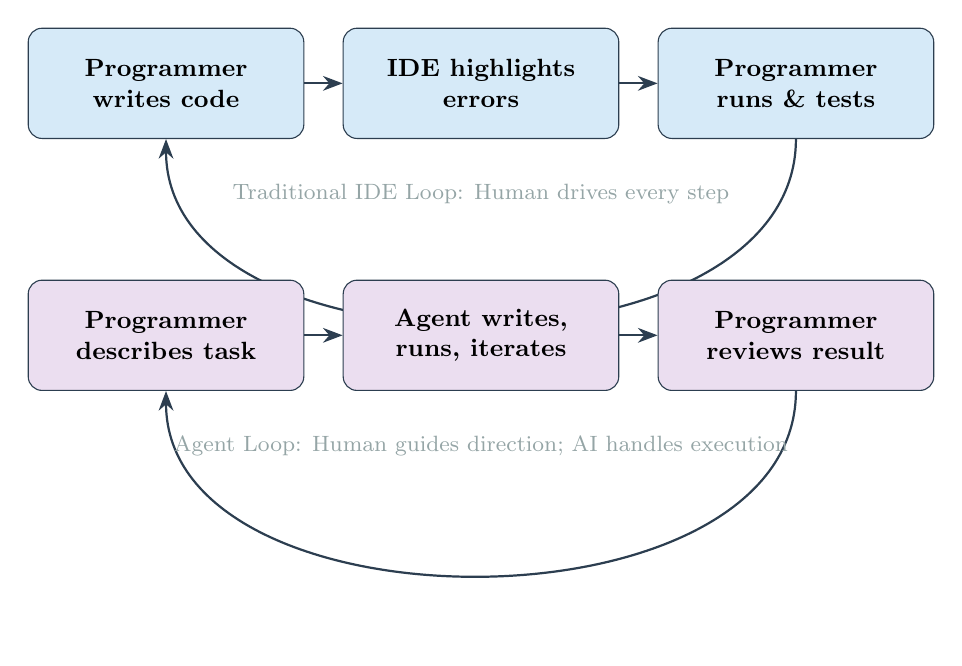
\begin{tikzpicture}[
    box/.style={rectangle, rounded corners=5pt, draw=csprimary, fill=#1, minimum width=35mm, minimum height=14mm, align=center, font=\small\bfseries},
    arrow/.style={-{Stealth[length=2.5mm]}, thick, color=csprimary},
    label/.style={font=\footnotesize, color=codegray, align=center}
]

% Traditional IDE loop
\node[box=cstertiary!20] (prog) at (0,0) {Programmer\\writes code};
\node[box=cstertiary!20] (ide) at (4,0) {IDE highlights\\errors};
\node[box=cstertiary!20] (run) at (8,0) {Programmer\\runs \& tests};

\draw[arrow] (prog) -- (ide);
\draw[arrow] (ide) -- (run);
\draw[arrow] (run.south) to[out=-90, in=-90] (prog.south);

\node[label] at (4,-1.4) {Traditional IDE Loop: Human drives every step};

% Agent loop
\node[box=codepurple!20] (task) at (0,-3.2) {Programmer\\describes task};
\node[box=codepurple!20] (agent) at (4,-3.2) {Agent writes,\\runs, iterates};
\node[box=codepurple!20] (review) at (8,-3.2) {Programmer\\reviews result};

\draw[arrow] (task) -- (agent);
\draw[arrow] (agent) -- (review);
\draw[arrow] (review.south) to[out=-90, in=-90] (task.south);

\node[label] at (4,-4.6) {Agent Loop: Human guides direction; AI handles execution};

\end{tikzpicture}
\end{center}

Tools like \textbf{Claude Code}, \textbf{Devin}, \textbf{SWE-agent}, and \textbf{OpenAI Codex} (distinct from the original) allow a programmer to say things like: ``Add input validation to all the form fields in this project,'' or ``Find and fix the bug that causes the tests to fail,'' and watch the agent do it---reading files, writing code, running tests, correcting mistakes.

\begin{quotebox}[What Interacting With an Agent Looks Like]
\small
\textbf{Programmer:} ``Our \texttt{StudentGrade} class doesn't handle the case where a student has no assignments. Add appropriate handling and write tests for it.''

\textbf{Agent:} \textit{[Reads \texttt{StudentGrade.java}, reads \texttt{StudentGradeTest.java}]}\\
``I see the issue---\texttt{calculateAverage()} divides by the list size without checking if it's empty. I'll fix this and add three new test cases.''\\
\textit{[Writes the fix, writes the tests, runs the test suite]}\\
``All 14 tests pass. Here's what I changed and why: [explanation]''

\textbf{Programmer:} ``The logic looks right, but use `Optional' for the return type instead of throwing an exception.''\\
\textit{[Agent updates implementation and tests]}
\end{quotebox}

This isn't science fiction. It's how many professional programmers are working today.

%---------- WHAT THIS MEANS FOR BEGINNERS ----------%
\section{What This Means for You as a Beginning Programmer}

\subsection{The Temptation and the Trap}

For a beginning programmer, AI tools are seductive---and that's worth thinking carefully about. If you can describe what you want and an AI writes the code, why learn to write it yourself?

The honest answer is that this is a real and open question. But there are good reasons to invest in understanding code deeply, even in an age of AI assistance.

\begin{debatebox}[The Understanding Gap]
AI tools work best when you can evaluate what they produce. When an AI generates code and it fails, you need to understand \textit{why} it's wrong. When an AI produces working code that's inefficient or hard to maintain, you need to recognize that.

More subtly: AI tools make mistakes. Sometimes the mistakes are obvious (a syntax error); sometimes they're subtle (a logic error that only triggers for edge cases; a security vulnerability that looks fine). A programmer who doesn't understand the underlying concepts can't catch these mistakes.

Beginning programmers who rely too heavily on AI tend to get stuck on problems the AI handles poorly: novel problems, unusual requirements, debugging AI-generated code that's broken in non-obvious ways.
\end{debatebox}

The analogy: knowing how to use a calculator is valuable, but students who skip learning arithmetic often struggle with algebra, because they lack a feel for whether answers make sense. Programming is similar. AI tools amplify your abilities---but if your abilities are thin, there's little to amplify.

\subsection{Practical Tips for Using AI Tools as a Beginner}

AI tools are genuinely useful for learning---if used thoughtfully.

\begin{tipbox}[Using AI to Learn Rather Than Just Get Answers]
\begin{itemize}[itemsep=4pt]
    \item \textbf{Ask for explanations, not just code.} Instead of ``Write a method to sort this list,'' try ``Write a method to sort this list \textit{and explain each line}.'' Reading the explanation teaches you the pattern.

    \item \textbf{Predict before you accept.} When AI suggests a completion, pause and think: what do I expect this code to do? Then accept it, run it, and check your prediction. This builds the habit of reading code critically.

    \item \textbf{Type it yourself first.} Try solving the problem before asking AI for help. Even if you only get partway, you'll understand the AI's answer better for having struggled.

    \item \textbf{Use AI to debug, not to avoid understanding.} If your code is broken, describe the bug to an AI and ask it to help you understand what's wrong---not just to fix it for you.

    \item \textbf{Review AI output like code review.} Treat AI-generated code the way a professional treats a colleague's code: read it, understand it, and question anything that seems wrong or unclear.
\end{itemize}
\end{tipbox}

\subsection{VS Code Is Not Dead}

You might come away from this case study thinking: if agents are the future, should I even bother learning VS Code? The answer is unambiguously yes---for several reasons.

\begin{conceptbox}[Why VS Code Still Matters]
\textbf{Agents live inside IDEs.} GitHub Copilot, Cursor, and most other AI tools are either VS Code extensions or editors built on VS Code's codebase. Learning VS Code means learning the environment where AI tools live.

\textbf{You still write code.} Even with AI assistance, programmers spend significant time reading, understanding, and making targeted edits to code. An IDE makes all of this faster.

\textbf{The debugger is irreplaceable.} No AI tool makes the debugger less valuable. When something goes wrong---and things will go wrong---being able to pause execution and inspect state is essential.

\textbf{Skills transfer.} VS Code fluency---keyboard shortcuts, extensions, Git integration, the terminal---transfers to professional settings. Knowing your tools is a professional baseline.

\textbf{The agent era is early.} AI agents are impressive but imperfect. They make mistakes, get confused about requirements, and need human oversight. For the foreseeable future, programmers who understand the code will be more effective than those who don't.
\end{conceptbox}

%---------- THE BIGGER PICTURE ----------%
\section{The Bigger Picture: What is the Programmer's Role?}

\subsection{Tools Always Change the Work}

The history of programming tools is a history of raising the level of abstraction. Early programmers wrote in binary machine code---literally sequences of 0s and 1s. Assembly language let them write \texttt{ADD R1, R2} instead. High-level languages like Fortran and COBOL let them write something resembling math. Object-oriented languages let them model concepts directly. And now AI tools let them describe intent in natural language.

Each step up the ladder of abstraction made programmers more productive---and shifted the valuable skill from \textit{knowing the details} toward \textit{knowing what to build and whether it's right}.

\begin{center}
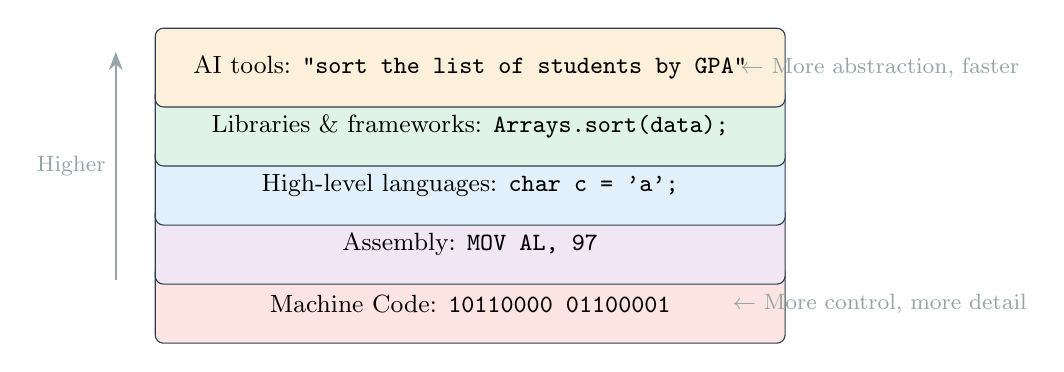
\begin{tikzpicture}[
    level/.style={rectangle, rounded corners=3pt, draw=csprimary, fill=#1, minimum width=80mm, minimum height=10mm, align=center, font=\small},
    label/.style={font=\footnotesize, color=codegray}
]
\node[level=cssecondary!15] (l1) at (0,0) {Machine Code: \texttt{10110000 01100001}};
\node[level=codepurple!15] (l2) at (0,0.75) {Assembly: \texttt{MOV AL, 97}};
\node[level=cstertiary!15] (l3) at (0,1.5) {High-level languages: \texttt{char c = 'a';}};
\node[level=csaccent!15] (l4) at (0,2.25) {Libraries \& frameworks: \texttt{Arrays.sort(data);}};
\node[level=cswarm!15] (l5) at (0,3.0) {AI tools: \texttt{"sort the list of students by GPA"}};

\draw[-{Stealth}, thick, color=codegray] (-4.5,0.3) -- (-4.5,3.2) node[midway, left, font=\footnotesize, color=codegray] {Higher};
\node[label] at (5.2,0) {$\leftarrow$ More control, more detail};
\node[label] at (5.2,3.0) {$\leftarrow$ More abstraction, faster};
\end{tikzpicture}
\end{center}

The programmer's role shifts with each level. At the machine-code level, you must understand every bit. At the AI level, you must understand what you want to build, how to evaluate whether it's built correctly, and how to guide the AI when it goes wrong.

\subsection{New Skills for the Agent Era}

If AI tools handle more of the typing and routine problem-solving, which skills become more valuable?

\begin{itemize}[itemsep=4pt]
    \item \textbf{Problem decomposition:} Breaking a large, vague task into small, concrete steps that an AI (or a human) can execute. This is a skill that must be learned and practiced.

    \item \textbf{Code reading and review:} Understanding unfamiliar code quickly---knowing what a function does, spotting subtle bugs, recognizing bad patterns. This is harder to fake with AI assistance.

    \item \textbf{System design:} Deciding how pieces fit together---which classes to create, how components communicate, what data model to use. AI can suggest, but humans must judge.

    \item \textbf{Testing and verification:} Knowing what ``correct'' means and how to verify it. Writing good tests remains a high-value skill even if AI writes the implementation.

    \item \textbf{Communication:} Describing requirements clearly---to teammates, to AI agents, and to stakeholders. Vague requirements produce vague (and wrong) results.
\end{itemize}

\begin{debatebox}[Will AI Replace Programmers?]
This question comes up constantly, and the honest answer is: partially, and unevenly.

Routine, well-defined coding tasks---writing boilerplate, translating specifications into standard patterns, fixing common bugs---are increasingly automatable. Some entry-level roles that consisted primarily of these tasks may shrink.

But programming is not just writing code. It involves understanding users' real needs (which they often can't fully articulate), making design decisions with long-term consequences, evaluating tradeoffs, and ensuring correctness. These remain stubbornly human-centered activities.

More likely than replacement: the \textit{kind} of programmer work changes. Professionals who learn to work effectively with AI tools---directing, reviewing, and correcting AI-generated code---will be more productive than those who don't. The skill of working \textit{with} AI is itself becoming a professional competency.
\end{debatebox}

%---------- PRACTICAL GETTING-STARTED GUIDE ----------%
\section{Getting Started: Your Recommended Setup}

If you're just beginning, here's a practical path that prepares you for both the current landscape and where things are heading.

\begin{tipbox}[Your Recommended Development Setup]
\textbf{Step 1: Learn VS Code.}
Download it free at \texttt{code.visualstudio.com}. Install the Java Extension Pack. Spend time learning:
\begin{itemize}[itemsep=1pt]
    \item Basic keyboard shortcuts (Ctrl+P to find files, Ctrl+Shift+P for commands)
    \item How to set breakpoints and use the debugger
    \item The integrated terminal (\texttt{Ctrl+`})
\end{itemize}

\textbf{Step 2: Learn Git basics.}
Git is non-negotiable in professional software development. Learn to \texttt{init}, \texttt{add}, \texttt{commit}, \texttt{push}, and \texttt{pull}. Set up a free GitHub account and push your projects there.

\textbf{Step 3: Try an AI assistant---carefully.}
GitHub Copilot offers a free tier for students. Install it in VS Code and experiment. Use it to explain code you don't understand, suggest completions for patterns you half-remember, and generate test cases. Watch it make mistakes. Ask it to explain its reasoning.

\textbf{Step 4: Build projects you care about.}
The best way to learn any tool is to use it for a real goal. Build something you actually want: a grade calculator, a simple game, a tool that solves a problem you have. Tools make sense in context.
\end{tipbox}

%---------- DISCUSSION QUESTIONS ----------%
\section*{Discussion Questions}

\begin{questionbox}
\begin{enumerate}[leftmargin=*, label=\textcolor{cswarm}{\textbf{\arabic*.}}]
    \item \textbf{The Learning Paradox:} AI tools can write code that beginning programmers can't yet write themselves. Is this a good thing---a way to see correct solutions and learn from them---or a bad thing, because it bypasses the struggle that produces deep understanding? Where do you draw the line in your own learning?

    \item \textbf{The Abstraction Ladder:} Each step up the abstraction ladder (machine code $\to$ assembly $\to$ high-level languages $\to$ AI tools) made some skills obsolete while making others more valuable. What skills are we in danger of losing as AI writing code becomes common? Are there skills from earlier eras that we've already lost---and do we miss them?

    \item \textbf{The Review Problem:} A core argument for learning to code is that you need to review and verify AI-generated code. But if AI gets good enough, will human review remain meaningful? Could an AI review another AI's code? What would that mean for the human role?

    \item \textbf{The IDE as Interface:} The IDE gave programmers a powerful environment for working with code. The agent interface gives programmers a way to \textit{direct} code without necessarily writing it. What kinds of people might be better served by the agent interface than the IDE? Does this expand or contract who can participate in software development?

    \item \textbf{Your Own Practice:} How do you currently use (or plan to use) AI tools in your own programming? What guardrails or habits do you think you need to develop to make sure these tools enhance rather than substitute for your own understanding?
\end{enumerate}
\end{questionbox}

%---------- GLOSSARY ----------%
\section*{Key Terms}

\begin{glossarybox}
\begin{description}[leftmargin=!, labelwidth=3.6cm, font=\bfseries\color{cssecondary}]
    \item[Agent] An AI system that can autonomously perform multi-step tasks: reading files, writing code, running programs, and fixing errors---without requiring a human to drive each step.

    \item[Autocomplete] An IDE feature that suggests completions for the code you are typing, based on the available methods, variables, and libraries.

    \item[Breakpoint] A marker placed in code that causes a debugger to pause execution at that line, allowing inspection of program state.

    \item[Debugger] A tool that lets programmers pause a running program, inspect variable values, and step through code line by line to find errors.

    \item[Edit-Compile-Run Cycle] The fundamental loop of programming: write code, compile it, run it, observe the results, and repeat.

    \item[Git] A version control system that tracks changes to code over time, enabling history, collaboration, and the ability to revert to earlier versions.

    \item[GitHub Copilot] An AI-powered code assistant (by GitHub and OpenAI) that suggests code completions and generates entire functions from natural-language descriptions.

    \item[IDE] Integrated Development Environment; an application combining a code editor, compiler, debugger, and other tools in a single interface.

    \item[IntelliSense] Microsoft's name for the smart autocomplete feature in VS Code, which shows method signatures, documentation, and context-aware suggestions.

    \item[Modal Editing] Vim's approach to text editing, where the editor has separate modes for inserting text and for navigating and manipulating it.

    \item[Syntax Highlighting] Coloring different parts of code (keywords, strings, variables) to make structure immediately visible.

    \item[Version Control] A system for tracking changes to files over time, allowing reversion, comparison, and collaboration.

    \item[VS Code] Visual Studio Code; a free, extensible code editor by Microsoft, currently the most widely used editor among developers worldwide.
\end{description}
\end{glossarybox}

\vspace{5mm}

%---------- FOOTER ----------%
\begin{center}
\textcolor{csprimary}{\rule{0.6\textwidth}{0.5pt}}\\[3mm]
{\small\textcolor{gray}{This case study is part of the Open Educational Resources for \cscourse.\\
Licensed under Creative Commons Attribution 4.0 (CC BY 4.0).}}
\end{center}

\end{document}
